\documentclass[output=paper]{langsci/langscibook} 
\author{Christopher Lucas\affiliation{SOAS University of London}\lastand 
 Stefano Manfredi\affiliation{CNRS, SeDyL}
}
\title{Introduction}
% \keywords{} 
\abstract{Abstract}
\maketitle

\begin{document}

\section{Rationale}
Expand and edit the proposal text:
This proposal is for a handbook-style volume focused on the topic of contact-induced change in the history of both Arabic and its contact languages. As well as a brief introduction, the volume will include approximately 30 short (c.5000-word) chapters authored by invited experts, falling into the following three categories: overviews of contact-induced change in individual Arabic varieties; overviews of the outcomes of contact with Arabic in other languages; and overviews of various types of changes across Arabic varieties, in which contact has played a significant role.
Chapters in each of the three categories will follow the fixed broad outlines detailed below, to ensure coherence and ease of reference. All authors have also been encouraged a) to ensure their chapters contain a rich set of linguistic data, including original data where appropriate, and b) to frame their presentation where possible with reference to Van Coetsem’s (1988, 2000) distinction between changes due to borrowing (by agents dominant in the recipient language) and imposition (by agents dominant in the source language). 
The proposed volume would be the primary output of the recently awarded AHRC Leadership Fellows project ‘Arabic and contact-induced language change’. A key aim of this project, and the primary rationale of the volume, is to showcase the current state of knowledge regarding the diverse outcomes of contacts between Arabic and other languages, in a format that is both accessible and useful to scholars and students of historical linguistics who are not specialists in Arabic. We intend to achieve this by making sure chapters provide both ample uniformly glossed and transcribed linguistic data, and as much sociohistorical data as possible on the speech communities involved in the changes, organised in terms of Van Coetsem’s framework. The latter feature is aimed at ensuring that the data presented in the volume can be productively drawn upon by linguists working on the mechanisms, typology, outcomes and theory of contact-induced change cross-linguistically.
Our contention is that Arabic – with its lengthy written history, wide and well-studied dialectal variation, and involvement in numerous heterogeneous contact situations – has considerable potential to deepen and broaden our understanding of the workings of contact-induced change in general. This potential has thus far barely been realised, however. Currently, most of what is known about the diverse outcomes of contacts between Arabic and other languages remains inaccessible to non-specialists; there are brief summary sketches (Thomason 2006, Versteegh 2001, 2010) but no larger synthesis of the kind that is available, for example, for Amazonian languages (Aikhenvald 2002). Arabic has thus played little part in work to date on contact-induced change that is crosslinguistic in scope (though see Matras 2009, Trudgill 2011 for partial exceptions). 
In sum, the proposed volume aims to rectify this situation by creating a collaborative synthesis of current expertise on contact-induced change in Arabic and its neighbours, so that linguists of all backgrounds can benefit from this particularly valuable and under-exploited resource.

We have invited contributions from a wide range of scholars with proven expertise in one or more of the areas we want the volume to cover. The final list of chapters in the volume will inevitably reflect a compromise between several different academic and practical considerations. For instance, we have aimed for blanket coverage of languages and varieties of Arabic that have been significantly affected by contact, but for some varieties (e.g. Yemeni Arabic dialects) it has not yet been possible to recruit a scholar with sufficient expertise to contribute a chapter. Where blanket coverage has not been possible, we have generally sought to focus on those individual varieties and dialect areas that have been most intensively affected by contact (e.g. Maltese, Maghrebi Arabic in general, Domari), while not also excluding languages and varieties where contact influence has been milder (e.g. Mande languages, Gulf Arabic), but for which we have experts ready to contribute chapters.




\section{Existing work on Arabic and contact-induced change}
...

\section{A dominance-based approach to contact-induced change}
Introduce Van Coetsem's model.

\subsection{Imposition}
Example changes in the volume that are SL-agentivity based

\subsection{Borrowing}
Example changes in the volume that are RL-agentivity based

\subsection{Problematic cases}
...

\section{Alternative approaches to contact-induced change} 
...

\section{What and where is Arabic?}

\begin{figure}
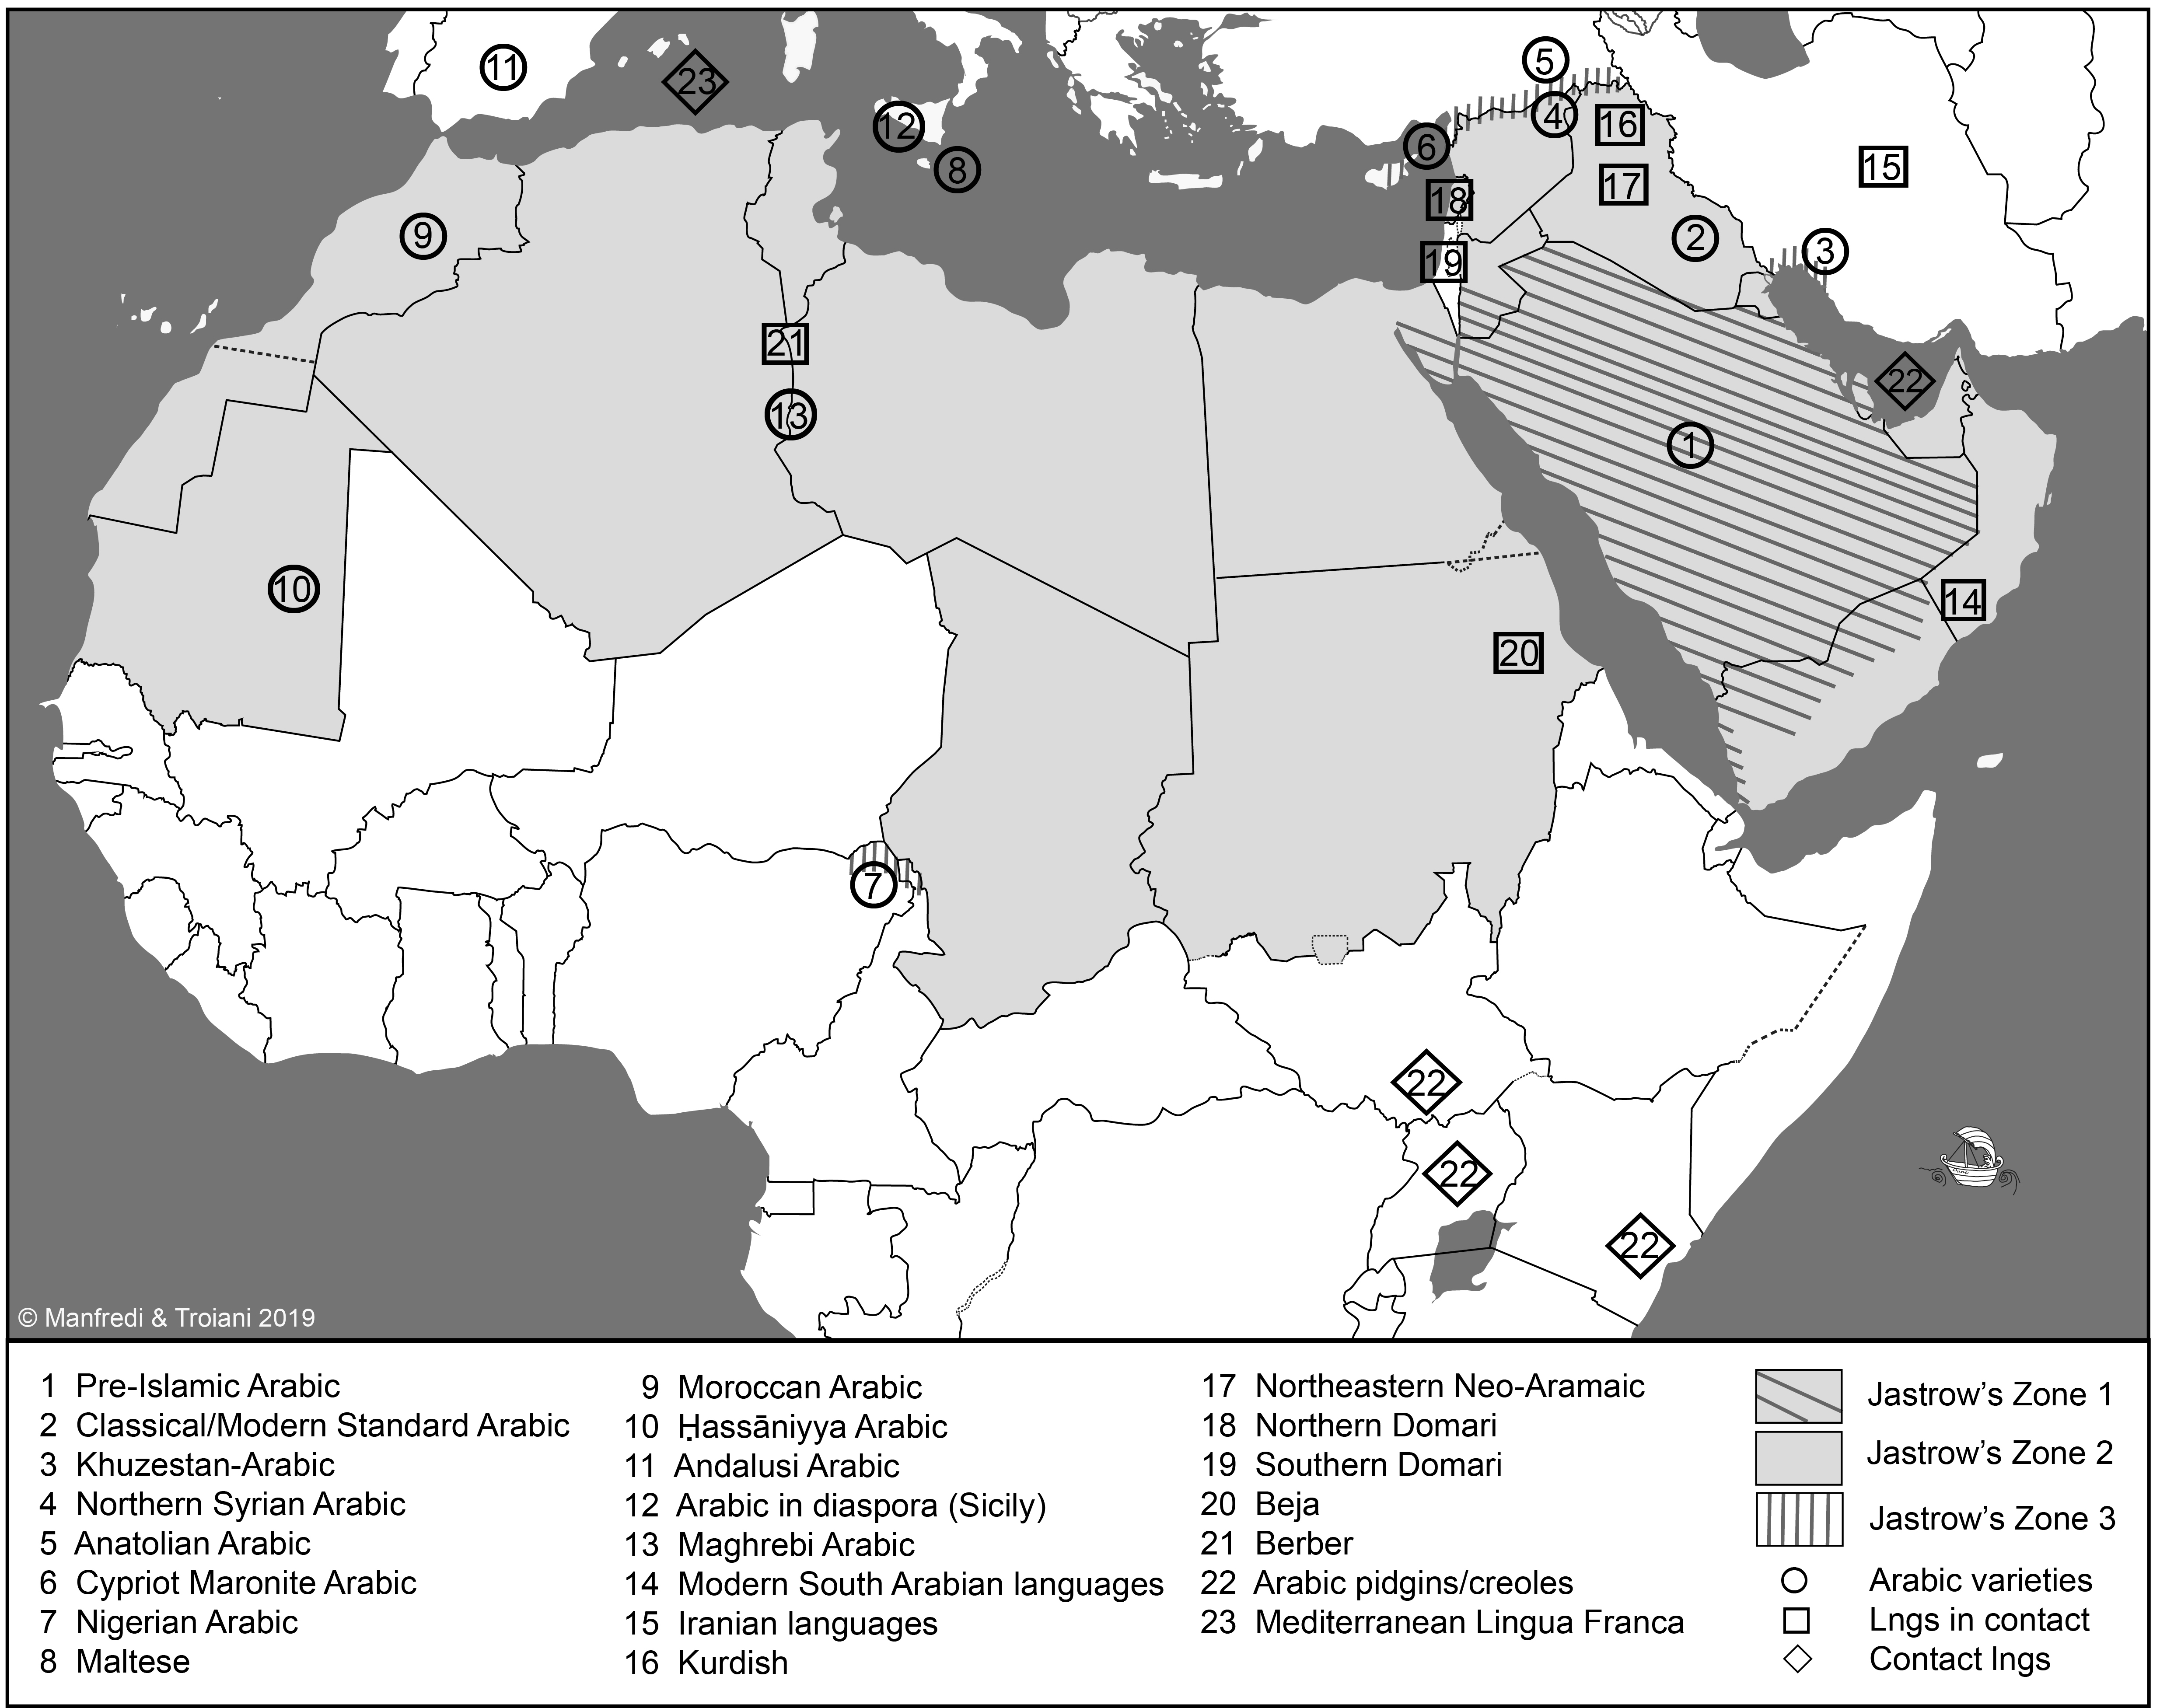
\includegraphics[width=\textwidth]{figures/Monde_arabe.jpg}
\caption{Map small and standard orientation}
\label{map}
\end{figure}

...
  
\begin{figure}
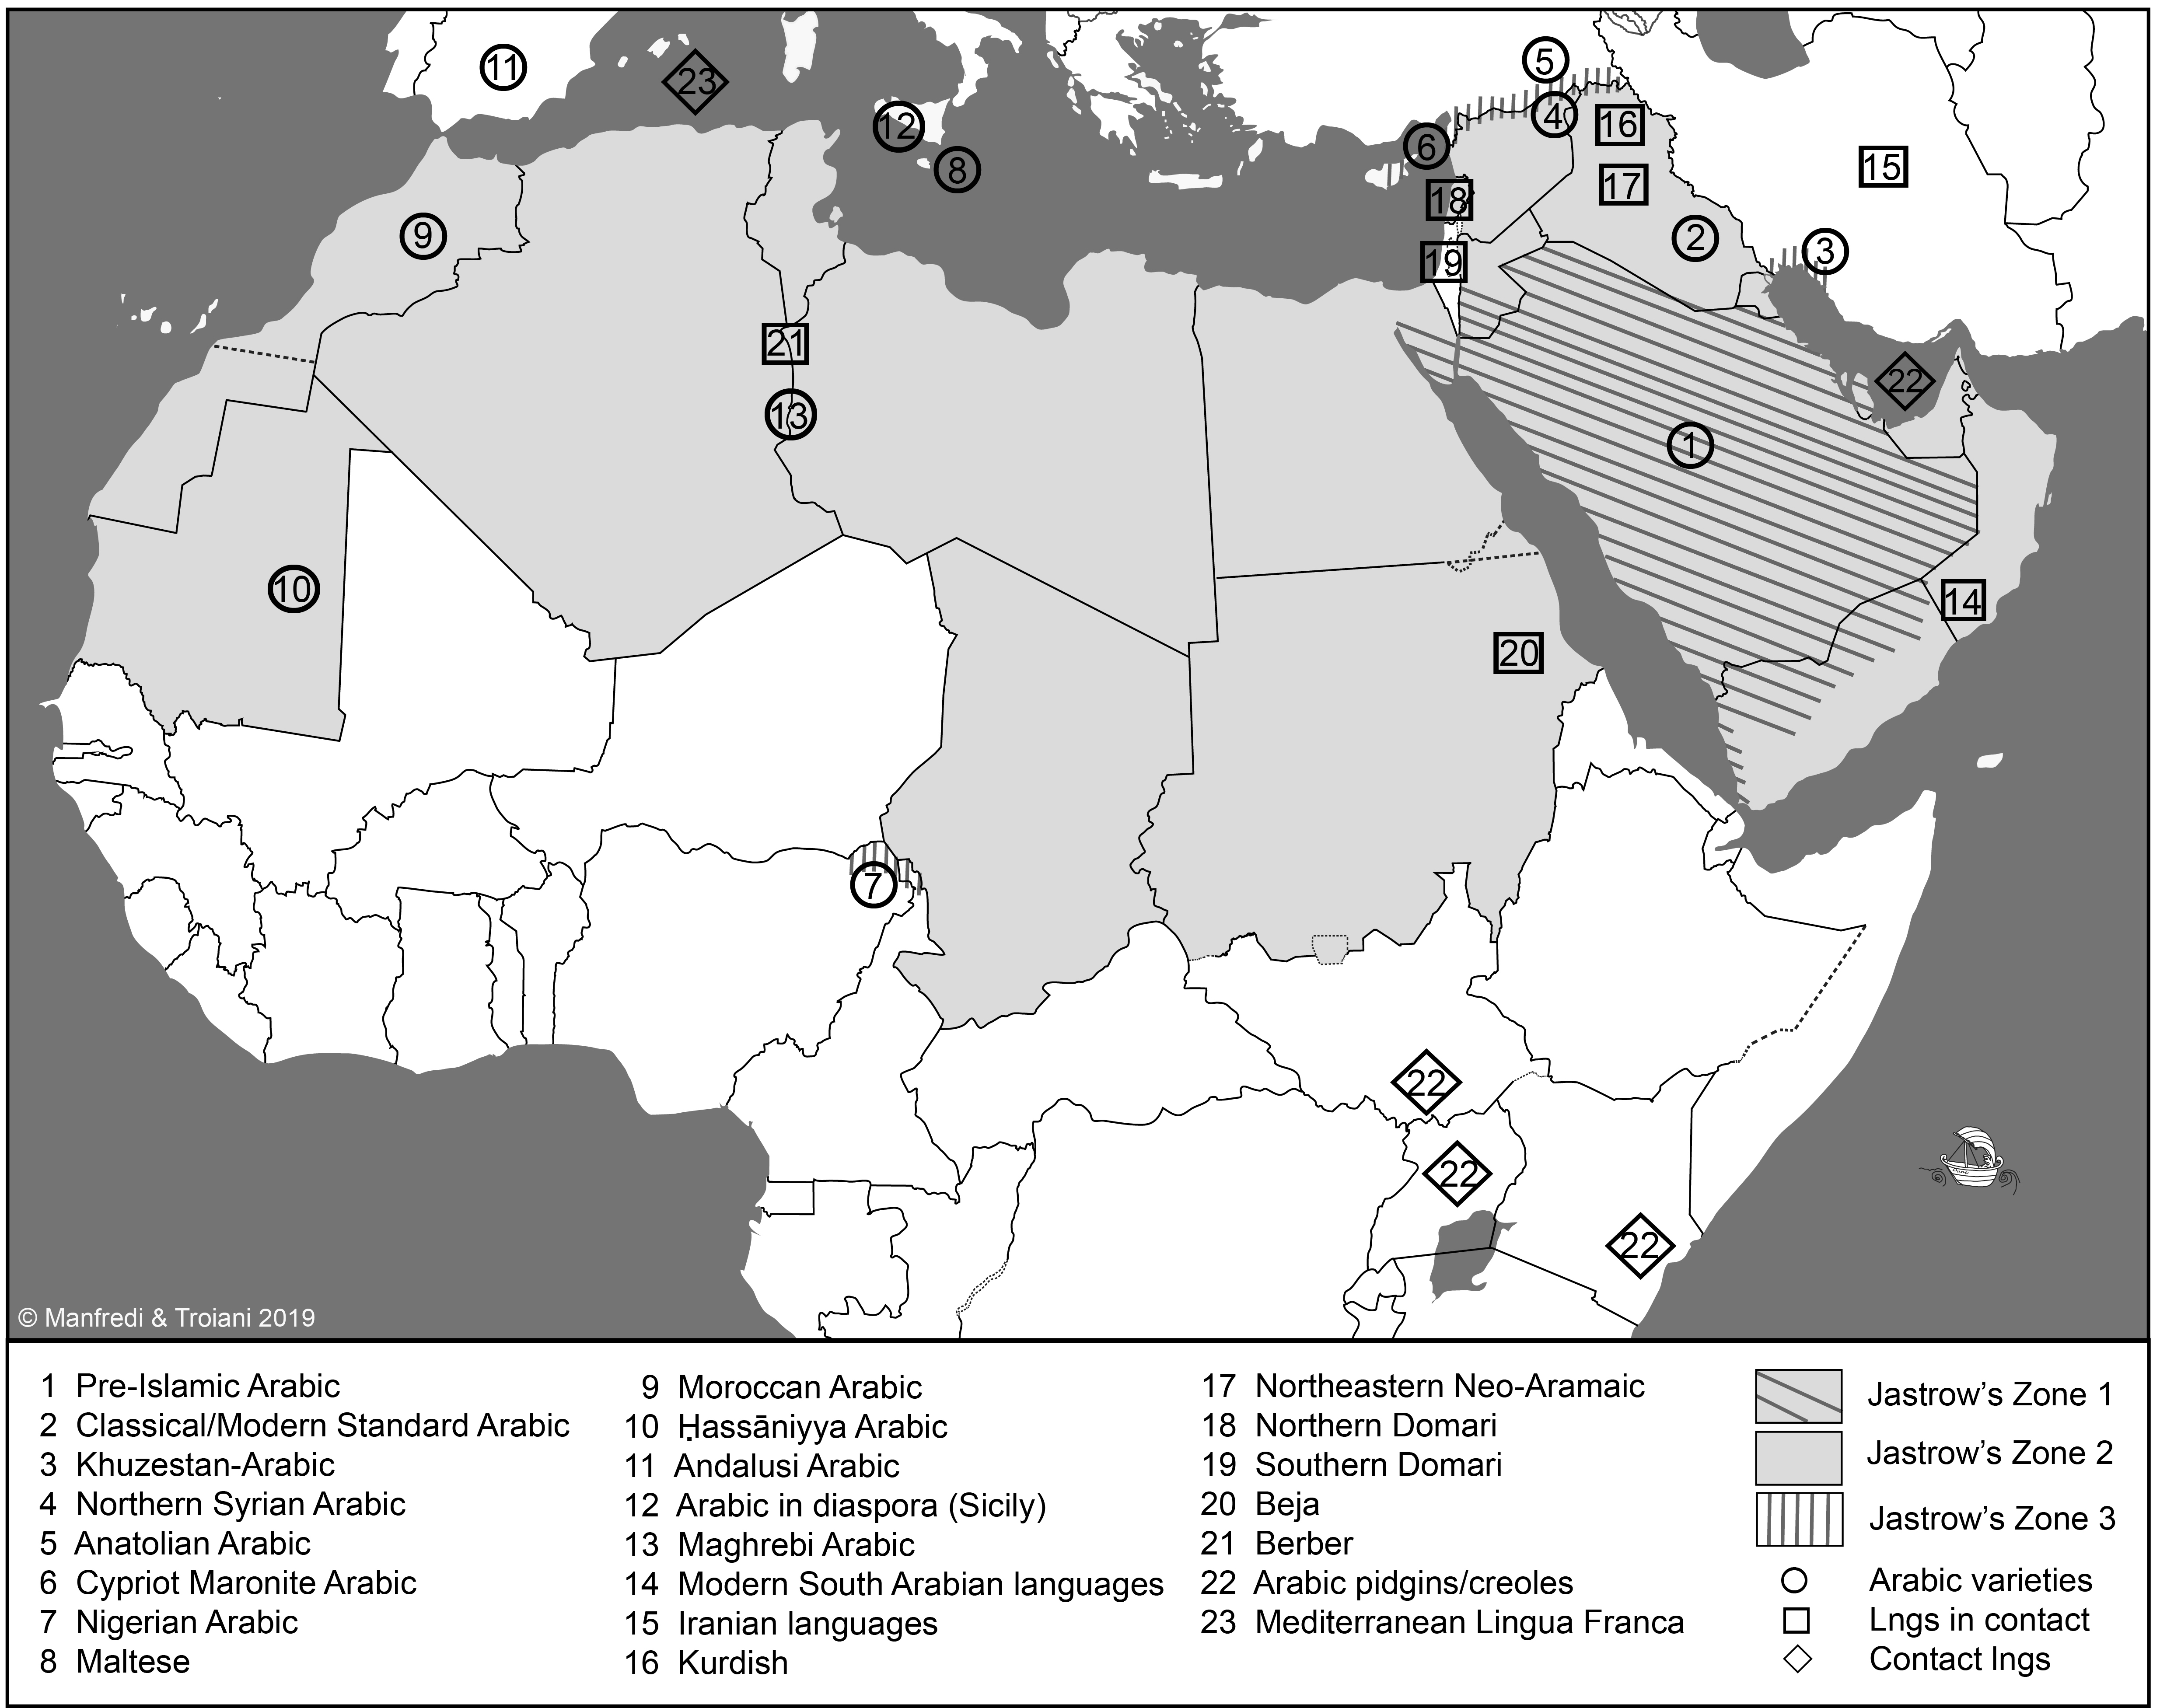
\includegraphics[height=.66\textheight, angle=90]{figures/Monde_arabe.jpg}
\caption{Map large and rotated orientation.}
\label{map}
\end{figure}


\section{Languages in contact with Arabic}
...

\section{The structure of the present work}
...

\section{Major themes of the present work}
...

\section{Future directions}
...

\section*{Abbreviations}

Some references:\\
\\
\citet{Jastrow2002}\\
\citet{Owens2000editor}\\
\citet{Owens2018}\\
\citet{Watson2011dialectsoverview}



\sloppy
\printbibliography[heading=subbibliography,notkeyword=this] 
\end{document}